{\color{reviewA}
\presub
\subsection{Evaluation on Distributions and Arrival Orders} \postsub
\label{eva_data}

\begin{figure}[!ht]
	\centering
	\subfigure[Impact of dataset distribution]{
		\begin{minipage}[t]{0.22\textwidth}{
			\prefig
			\begin{center}
			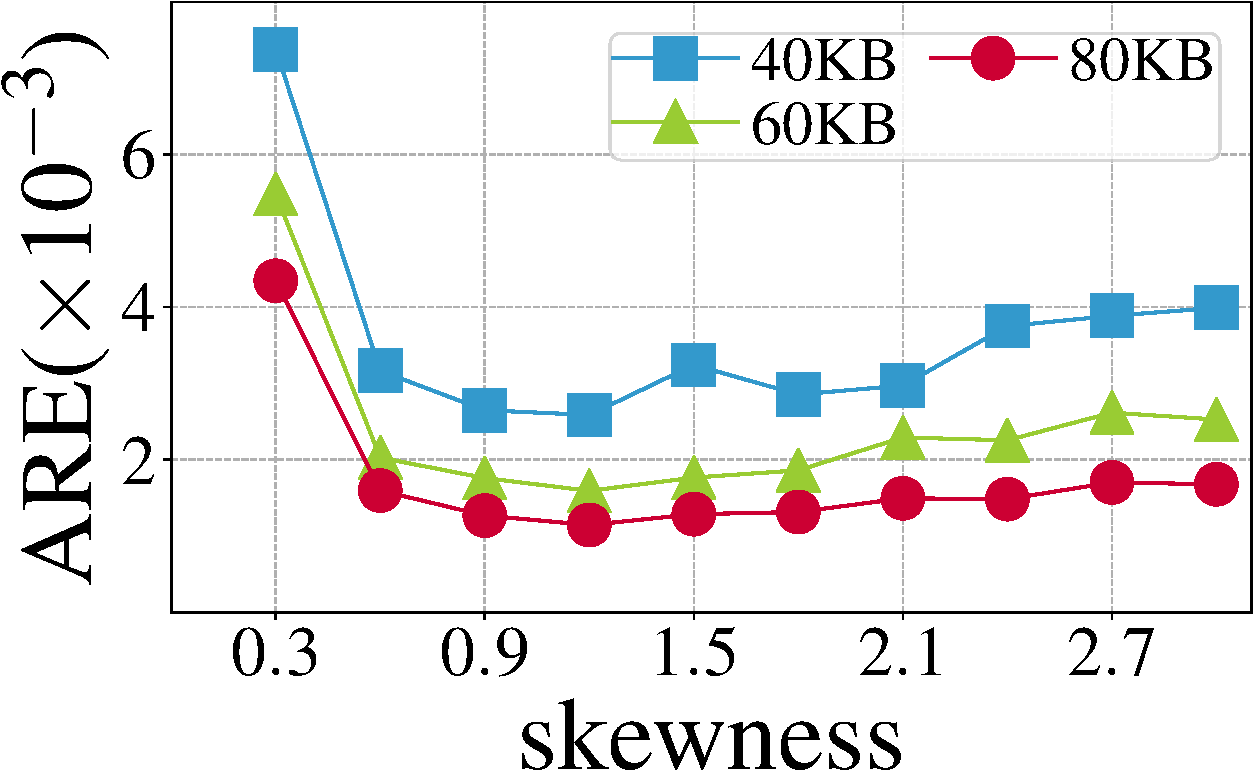
\includegraphics[width=\textwidth, ]{Figures/dataset/skew_out_are-cropped.pdf}
			\end{center}}
			\postfig 
			\adjustfigs
			\prefigcaption
			\label{skew_are}
			\postfigcaption
		\end{minipage}
	}
	\subfigure[Impact of arrival order]{
		\begin{minipage}[t]{0.22\textwidth}{
		    \prefig
			\begin{center}
			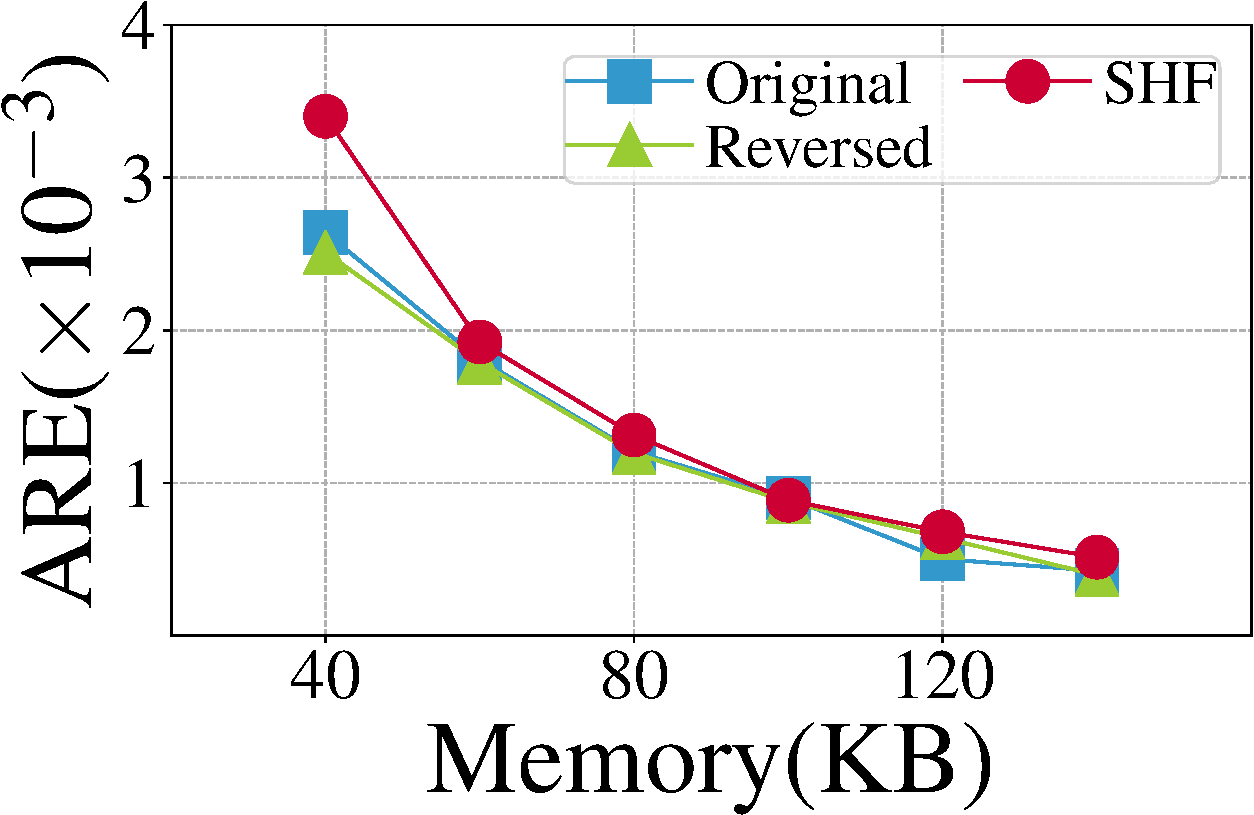
\includegraphics[width=\textwidth, ]{Figures/dataset/order_out_are-cropped.pdf}
			\end{center}}
			\postfig
			\adjustfigs
			\prefigcaption
			\label{order_are}
			\postfigcaption
		\end{minipage}}
	\vvv \vvv
    \caption{Accuracy vs. skewness and item arrival order. Given a dataset, ``SHF'' refers to that the Second Half of items go First.}
	\label{dataset}
\end{figure}

In this subsection, we show how the dataset distribution and the arrival order of items affect the accuracy of PRI.

\noindent\textbf{Parameter Setting:}
We use synthetic datasets whose skewness varies from 0.3 to 3.0 to show the impact of dataset distribution to InterestSketch. We use the dataset whose skewness is 1.5 and three different orders to show the impact of the arrival order of items. Three different orders are the original order, the reversed order, and the Second Half First (SHF).
%
In this experiment, we plot the change of ARE of InterestSketch to show the impact.
The size of memory used ranges from 40KB to 140KB. We choose this range because using small memory can clearly expose the impact.

\noindent\textbf{Impact of dataset distribution (Figure~\ref{skew_are}):}
Our results show that the ARE of \sketchname{} is often lower than 0.01, and changes a little bit, especially when skewness is larger than 0.6.

\noindent\textbf{Impact of arrival orders (Figure~\ref{order_are}):}
Our results show that arrival orders indeed make some effects on the ARE of our \sketchname, but the effect is also not significant.
Because PRI replaces the minimum counter with a probability, the fluctuation of ARE in a certain range is reasonable.
}
